\chapter{Introduction}
\label{chap:introduction}

The global flow of foreign direct investment (FDI) has risen from almost nothing
in the 1970s to over \$2.3 trillion dollars in 2016, becoming an important
source of global capital (Figure~\ref{fig:globalfdi}). For developing countries
especially, capital from multinational corporations (MNCs) is robust to global
economic downturns, prompting major international organizations to endorse FDI
as a key factor to economic development and poverty reduction
\citep{Mallampally1999, WorldEconomicForum2013}.\footnote{While FDI into
  developed economies dropped almost 50\% during the 2000 recession and the 2008
  financial crisis, FDI into developing countries only experienced a plateau or
  a small reduction. More recently, as global FDI flow slipped in 2016 and 2017,
  FDI into developing countries still remained stable \citep{UNCTAD2018}.} Within the scholarly
field of International Political Economy (IPE), much of the literature starts
with the view that countries will always seek FDI for its various benefits
\citep{Jensen2008b}. Works in IPE tend to focus on \textit{how} countries can
attract FDI, and do not question \textit{whether} they want to do so
\citep{Jensen2003, Li2003, Li2006, Ahlquist2006}.\footnote{Two recent exceptions
  are \citet{Pinto2013} and  \citet{Pandya2016}, who are the first to examine variation in
  countries' demand for FDI.}

\begin{figure}[tbp]
  \centering
  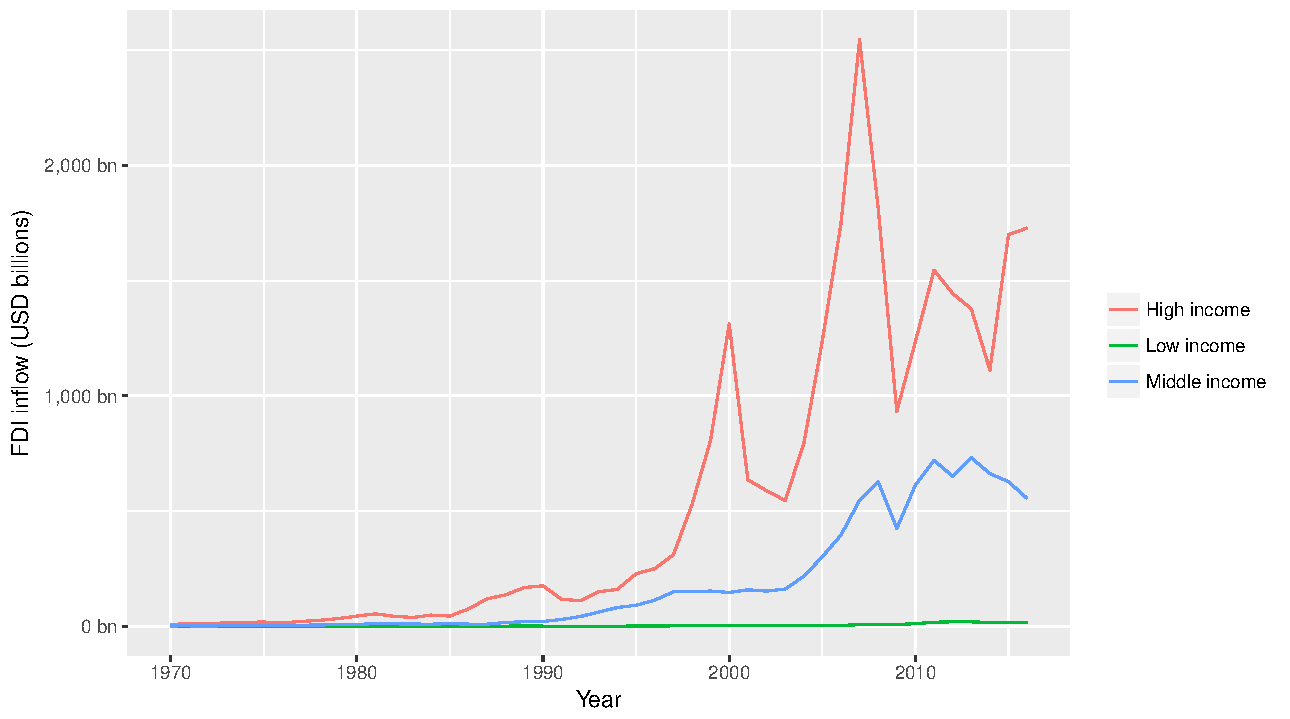
\includegraphics[width=0.8\textwidth,keepaspectratio]{../figure/global_fdi}
  \caption[FDI global inflow, 1970-2006.]{FDI global inflow, 1970-2006. The last
    four decades witness the growth of FDI into the most important source of
    global capital. Source: World Bank's World Development Indicators.}
  \label{fig:globalfdi}
\end{figure}

However, cross-country studies show that not all FDI are the same and that its effects are highly conditional. 

Given the evidence on the conditional effect of FDI, it is no longer tenable to
assume that countries' preference for FDI is homogeneous. By holding this
assumption, we neglect the role of the state in shaping global capital flow,
falling prey to the discredited ``race to the bottom'' thesis of globalization
\citep{Mosley2005}. Arguably, examining countries' preference for FDI should be
of more interest to political scientists than the current focus on determinants
of MNCs' location, which often amounts to adding a political variable to an
existing economic model of FDI flow. In addition, even if we only care about
MNCs' preference, to get an accurate estimate we must still take into account
countries' preference. For example, consider the received wisdom that
democracies receive more FDI \citep{Jensen2008a}. Without controlling for
countries' preferences, it is difficult to interpret this finding as democracies
actively pursuing MNCs or as MNCs finding democracies attractive.

\section{Benefits of FDI}

At first glance, the benefits of FDI seem obvious. FDI brings capital, creates
jobs, contributes tax revenue, and promises technological spillover to the local
economy. Consider the impact of an Intel's factory on Vietnam's economy. In
2006, Intel chose Saigon Hi-tech Park in Ho Chi Minh City as the site for its
largest chip testing and assembly in the world. From the initial plan of a \$300
million facility, Intel decided eight months later to increase the investment to
\$1 billion dollar, making up almost 10\% of Vietnam's registered FDI in 2006.
In 2016, Intel Products Vietnam (IPV) employed 4000 workers at full capacity,
exported \$3.45 billion worth of goods (or 18.2\% of Vietnam's electronics
export), and generated more than \$100 million for Vietnam's GDP in tax payment,
salary, and profit. In addition, IPV contributed to Vietnam's long-term
growth by addressing Vietnam's skill shortage in engineering and management. In
the first years, IPV had to improvise, hiring workers earlier and training them
at other Intel facilities in Asia. Later on, IPV developed an engineering
education program in partnership with Arizona State University and local
universities, educating and hiring thousands of young Vietnamese engineers. As a
result, IPV's workers were vastly more productive. While IPV's workforce only
constituted 5\% of all workers, its export value amounted to 72\% of all export
at the Saigon Hi-tech Park. Finally, Intel's decision to choose Ho Chi Minh City
over other candidate sites, including Chennai (India), Bangkok (Thailand), and
Dalian (China), was a significant marketing boost to Vietnam's image as a
destination capable of high-tech manufacturing. Following Intel, many other MNCs
opened high-tech facilities in Vietnam, including Samsung's three factories (in
2009, 2013, and 2014), Nokia/Microsoft (2012), and LG (2013) \citep{Dinh2016,
  UNCTAD2008}.

Economists have also theorized about the benefits of FDI for a long time. For
example, \citet{Findlay1978} argues that FDI plays a key role in economic growth
by upgrading the local economy's technological capability. As well-known from
neoclassical growth theory, diminishing returns to capital will at one point
stop capital from accumulating further, preventing long-run economic growth from
being driven by capital accumulation alone \citep{Solow1956}. FDI can counteract
this dynamic by helping local workers and suppliers upgrade their productivity,
either via training or demonstration. In other words, technological spillover
from FDI shifts the domestic factor-price frontier to the right, resulting in a
continually increasing capital stock and sustained economic growth.

For example, there is no conclusive evidence of FDI inflow having a positive effect on
growth \citep{Nair-Reichert2001, Carkovic2002} or poverty reduction
\citep{Guerra2009}. This puzzle opens a substantial literature on how the
growth-enhancing and spillover effect of FDI is conditional on the absorptive
capacity of the host economies, i.e. its level of human capital, technological
sophistication, and financial market development \citep{Durham2004,
  Nunnenkamp2004, Fu2008, Willem2004}. In addition, while the capital brought
and jobs created by FDI may be unconditionally good for the overall economy, its
distributional effects cut across constituencies in the host economy, creating
political cleavage across both sectoral and geographical divides
\citep{Chintrakarn2012, Goldberg2007, Nunnenkamp2007}.

\section{Goal of the research}

My research aims to estimate the preference of countries and MNCs for each
other. I develop an empirical strategy that takes into account the two-sided
nature of the FDI market, i.e. a subsidiary can only materialize if both the MNC
and the host government agree. Recognizing that this two-sided matching dynamics
can also be found in the labor or the marriage markets, I adapt the statistical
models first developed in Sociology for labor and marriage markets and apply
them to the study of FDI \citep{Logan1996, Logan2008}.

In doing so, I simultaneously address three long-standing issues in the FDI
literature. First, I ``bring the state back in,'' filling the gap in the literature on the
variation of countries' preference for FDI.\footnote{\citet{Evans1985}'s
book argues that states are weighty actors with their own capabilities and
initiatives rather than an arena for societal and interest groups to negotiate
for their share. Here, I argue that states are weighty actors with their own
preferences rather than goods that MNCs pick and choose.} Two notable exceptions are
\citet{Pinto2013} and \citet{Pandya2016}, whose pioneering works propose
partisan politics and regime types as factors shaping preferences for FDI.
However, while their theories are ground-breaking, the empirical estimation of
countries' preference remains inadequate. In addition, these researchers have
not used their findings to re-estimate the preference of MNCs and disentangle
the ``push'' and ``pull'' factors of FDI flow.\footnote{``Push factors'' refer
  to characteristics of the home country and of the MNC, pushing capital out
  from its origin. ``Pull factors'' refer to the characteristics of the host
  country, pulling capital towards its destination.} Using a two-sided matching
model, I will naturally be able to estimate both sides' preference.

Second, I propose that we need to pay more attention to countries' preference
for different types of FDI. While the IPE literature has largely focused on the
quantity of FDI flow, countries pay much attention to the its type, using
various incentives and restrictions to target certain types of FDI. Indeed, MNCs
come with varying amount of capital, labor demand, and technological
sophistication, all of which have different effects on the host country's
economy. Just as the two-sided matching model can estimate MNCs' utility
function for countries' characteristics (e.g. market size, level of
development), it can also estimate countries' utility function for MNCs'
characteristics (e.g. technological sophistication, export strategy).

Third, while the majority of the literature uses FDI flow data, these data
are accounting constructs created to keep track of countries' balance of payment
and thus map poorly to concepts in Political Science theories. Very often, the
variable of interest in our theories is the scale of MNCs' activities in the
host country, which can be very different from the amount of border-crossing
capital thanks to MNCs' complex financial and tax strategies \citep{Kerner2014}.
Therefore, we would do much better testing our theories with firm-level
operational data. Because the two-sided matching model is a behavioral model in
which each actor's decision is a unit of observation, and we can naturally use
it to analyze firm-level data.

These three issues are related and represent the status quo in the FDI
literature. Data limitation forces scholars to look at country-level aggregate
FDI flow, making it difficult to study countries' preference for FDI types. And
without studying countries' preference, our current models of MNCs' location
choice are also suspect.

In sum, my dissertation benefits the field by using firm-level data to estimate
both firms' and countries' preference for each other's characteristics. In this
two-sided matching model, MNCs and countries evaluate their available options
according to their utility functions, choose the best alternative, culminating
in an MNC's subsidiary located in a host country.

Estimating this model would be straightforward if we observed not only
subsidiaries' locations but also their set of options (called their
``opportunity set'' in the matching literature).\footnote{Discrete choice models
  can be used to estimate the utility function when both the choice and the set
  of options are observed. Indeed, discrete choice models remain the dominant
  empirical approach in the industrial location literature, effectively ignoring
  the fact that not all MNCs have the same set of location options
  \citep{Arauzo-Carod2010}.} Unfortunately, while data on subsidiaries' location
are available, the opportunity set is generally unobserved as researchers cannot
peek into the negotiation process between countries and MNCs. The two-sided
matching model solves this problem by using the Metropolis-Hastings (MH)
algorithm, a Markov chain Monte Carlo (MCMC) approach that repeatedly samples
new opportunity sets and rejects them at an appropriate rate to approximate
their true distribution. In addition, the estimated preference parameters in the
two-sided model have a convenient interpretation as the relative weight of
different variables on MNCs' and countries' utility. This allows us to make
statements such as: ``In evaluating MNCs, China values a 2\% increase in the
firm's capital as much as a 1\% increase in labor demand.''

\section{Benefits of the research}

During my time at the World Bank, an official opined that many of his country
clients needed help with formulating their FDI attraction policies. Regardless
of their situations, most country clients want to increase their FDI inflow, ideally in high-tech industries, relying on fiscal incentives such as tax holiday, land
concession, or lower utility price. Economists tend to look askance at such
heavy-handed industrial policies. Rather than encouraging governments to pick
winners, the World Bank gives governments the sanctioned advice of getting the
fundamentals right, i.e. liberalizing trade and investment, upholding rule of
law, eradicating corruption, and upgrading its labor force. Perhaps not
coincidentally, most of the FDI literature has also focused on studying what
country characteristics are attractive to MNCs, settling on the same familiar
list of desirables.

These approaches veer towards the extremes, one trusting and the other
discarding industrial policies entirely. At the same time, they are also
similar: both neglect the fact that a country's FDI inflow depends not only on
its policies but also the competitive landscape that in which it is situated. In
formulating their FDI strategies, a country's policy makers should neither
unilaterally determine what sectors do they want, nor abstractly ask what macro
conditions are associated with FDI inflow. Rather, they are better off
thinking strategically about realistic scenarios. For example, given China's rising
wage and tougher environmental regulations, how much and what type of FDI will
look to diversify out of China? What share of that flow can our country capture
at the current condition? How much can we capture if we increase the
productivity of our labor force by 5\% or 15\%? How much can we capture if other
countries also increase their GDP per capita by 10\% in the mean time? My
research provides the tool for policy makers to answer such kind of questions,
which serve as a firmer foundation for strategizing FDI attraction. To quote Sun
Tzu's ``The Art of War'' (as the business community is apt to do), ``If you know
the enemy and yourself, you need not fear the result of a hundred battles.''

In other words, my research allows policy makers to formulate better informed
industrial policies as a middle ground between defeatism (``Industrial policies
don't work'') and a pipe dream (``We want high-tech FDI, so they will come'').
The time is right for such an approach. First, the opportunity is there to
target the FDI that China no longer attracts. As China becomes more expensive,
aims to move into high-tech manufacturing, and withdraws their preferential
treatment, MNCs are looking towards diversifying into other countries. In 2013,
an American lawyer in Phnom Penh said that ``Every couple days, I'm getting
calls from manufacturers who want to move their businesses here from China''
\citep{Bradsher2013}. By 2017, a quarter of AmCham China's survey respondents
reported that they had either moved operations out of China or were planning to
do so, nearly half of which to other parts of Asia \citep{AmCham2018}.

Second, there is a resurgent appetite for industrial policy among international
development organizations, mainly the World Bank, who not only provide advice
but also funding to country governments. For a long time, World Bank economists
disavow industrial policy so completely that even the East Asian miracle,
arguably the clearest example of state-led industrialization, was interpreted as
a result of ``market-conforming'' policies
\citep[355]{WorldBank1993}.\footnote{See \citet{Amsden1994} and
  \citet{Rodrik1994} for a forceful rebuttal. Indeed, the East Asian miracle,
  i.e. the rapid growth with equity of eight high-performing Asian economies
  (Hong Kong, Korea, Singapore, Taiwan, China, Indonesia, Malaysia, and
  Thailand), was a Rorschach test for the international development world.
  Looking at the same set of facts, some saw the state micro-manage the market,
  while others, like the World Bank, saw the state getting the macro conditions
  right.} However, since the appointment of Justin Yifu Lin in 2008 as the chief
economist, the World Bank has supported programs that aim to restructure the
economy towards high-value added sectors \citep{Wade2012}. These programs look
like industrial policies, talk like industrial policies, but are called
``Competitive Industries'' instead.\footnote{In an advertising brochure, the
  Competitive Industries practice described itself as ``Going beyond
  macroeconomic reform agenda to identify and address the real microeconomic
  barriers to the growth of industries with high economic and social benefits''
  and ``Intervening aggressively \ldots to enable those industries to seize
  their 'windows of opportunity' to grow, compete and generate inclusive,
  productive employment.'' \citep{WorldBank2011}. In recent years, the program
  has expanded into ``Competitive Industries and Innovation Program,'' a
  multi-donor partnership with the support of the World Bank, the European
  Union, and several donor governments. ``Industrial policy'' may still be a
  taboo at the World Bank, but ``competitiveness'' and ``innovation'' are fully
  embraced as they hide the state and highlight the private sector.} Purists at
the World Bank may remain skeptical, but operational economists and specialists
are enthusiastically onboard. Their daily job is to respond to countries'
borrowing request with funding and advice on how to spend it, and a development
program based on targeting specific industries provides ample opportunities for
lucrative advice-giving. Ten years after the first sign of resurgence, the
support for industrial policy, albeit under other names, has become mainstream.
Indeed, the director of Trade and Competitiveness, one of the World Bank's 14
global practices, exclaimed in an official blog post: ``FDI matters, but not all
FDI is created equal'' and promised to help countries target efficiency-seeking
FDI \citep{Fruman2016}.

\section{Roadmap}

In the rest of this introductory chapter, I review in-depth the three issues in
the literature of FDI's political determinants, outlining the current attempts
to address them and how my approach can contribute to the solution.

In Chapter~\ref{chap:model}, I describe the two-sided matching model, including
both its game-theoretic origin and its statistical estimation.
Chapter~\ref{chap:simulation} uses simulations to demonstrate the correctness of
the model and explore its characteristics. Chapter~\ref{chap:labor} applies the
model on US labor market data, the original domain of the two-sided matching
approach, in order to compare with and expand upon previous results.
Chapter~\ref{chap:FDI} brings us back to the study of FDI, applying the model on
firm-level data of Japanese MNCs in East and Southeast Asia.
Chapter~\ref{chap:conclusion} concludes and explores potential applications of
the two-sided matching model in other areas of Political Science.

%%% Local Variables:
%%% mode: latex
%%% TeX-master: "AnhLe_dissertation.tex"
%%% End:
